\section{Getting Started}

\subsection{What is uPrime?}

\href{https://cmdrryder.github.io/uPrime/}{uPrime} reads Tecplot \texttt{.dat} files exported from LaVision DaVis, and MATLAB \texttt{.mat} files containing PIV or CFD velocity fields. It provides a graphical interface for turbulence post-processing. You do not need to know Python, MATLAB, or any programming language to use it. Everything is point-and-click.

The workflow is always the same:
\begin{enumerate}[leftmargin=1.5em]
  \item Load your snapshots (\texttt{.dat} or \texttt{.mat}).
  \item Set the acquisition type and sampling frequency.
  \item Align the coordinate system if needed.
  \item Verify statistical convergence in the `Mean \& Convergence` module.
  \item Open any analysis module and explore your data.
\end{enumerate}

\subsection{What uPrime can do}

\begin{itemize}[leftmargin=1.5em]
  \item Load 2D2C and 2D3C (stereo) PIV data from multiple \texttt{.dat} files or a single \texttt{.mat} file.
  \item Display mean velocity fields, standard deviation, vorticity, velocity vectors, and streamlines.
  \item Plot mean velocity line profiles (free, horizontal, vertical) and verify cumulative-statistics convergence at any picked point.
  \item Compute all Reynolds stress components with 2D maps, line profiles, and uncertainty bands.
  \item Compute and plot the full TKE budget (production, convection, turbulent diffusion, residual) with selectable term visibility.
  \item Perform spatial, temporal, and space-time spectral analysis.
  \item Compute two-point spatial and temporal correlations with integral length and time scales.
  \item Analyze turbulence anisotropy via the Lumley triangle and barycentric maps (stereo only).
  \item Perform Proper Orthogonal Decomposition (POD) with energy spectra, mode shapes, and flow reconstruction.
  \item Perform Dynamic Mode Decomposition (DMD) with frequency spectra and spatial mode visualization (TR only).
  \item Identify vortex cores and boundaries using five scalar criteria: vorticity, Q-criterion, swirling strength, $\lambda_2$, and $\Gamma_1$/$\Gamma_2$ (Graftieaux).
  \item Compute probability density functions of the velocity components and their fluctuations at a point, along a line, in a region of interest, or over the whole field, with skewness and flatness.
  \item Map forward-flow and reverse-flow probability (backflow coefficient) to locate and quantify intermittent separation.
  \item Plot binary space-time maps of the fluctuation sign along a line to visualise the passage of coherent structures (TR only).
  \item Decompose the Reynolds shear stress into ejections, sweeps, and interactions by quadrant analysis, with a hole-size sweep and joint PDF.
  \item Import multiple cases (CSV) and overlay them in Reynolds stress, TKE budget, spectra, correlation, anisotropy, and mean velocity plots for direct visual comparison.
  \item Apply and manage non-destructive spatial masks.
  \item Correct camera calibration misalignment, shift the coordinate origin, and mirror the dataset.
  \item Export all results as Tecplot \texttt{.dat} or \texttt{.csv} files, and figures as PNG (300 DPI), PDF, or SVG with editable text.
\end{itemize}

\subsection{System requirements}

\begin{table}[htbp]
\centering
\caption{Minimum system requirements.}
\begin{tabular}{ll}
\toprule
\textbf{Item} & \textbf{Requirement} \\
\midrule
Operating system  & Windows 10/11 (primary); macOS 12+; Linux (Ubuntu 20+) \\
Python            & 3.10 or later (source installation only) \\
RAM               & 8\,GB minimum; 16\,GB or more recommended for large datasets \\
Display           & 1920$\times$1080 or larger strongly recommended \\
\midrule
\multicolumn{2}{l}{\textit{Python dependencies (source installation)}} \\
\midrule
\texttt{numpy}      & Array operations and numerical core \\
\texttt{scipy}      & Signal processing and spectral analysis \\
\texttt{matplotlib} & Plotting and figure export \\
\texttt{PyQt6}      & Graphical user interface \\
\texttt{pyfftw}     & Fast Fourier transforms (accelerates spectral analysis) \\
\texttt{h5py}       & Read v7.3 (HDF5-based) \texttt{.mat} files \\
\bottomrule
\end{tabular}
\end{table}

```{note}
All Python dependencies are installed automatically via \texttt{pip install -r requirements.txt}. The Windows executable requires no Python or dependency installation.
```

\subsection{Installation}

\subsubsection{Option A: Windows executable (recommended for non-developers)}

Download \texttt{uPrime\_v0.7.1.exe} from the
\href{https://github.com/CmdrRyder/uPrime/releases}{GitHub Releases page}
and double-click to launch. No Python or any other software is required.

```{note}
Windows Defender may show a security warning on first launch. Click \textbf{More info} then \textbf{Run anyway}. This is normal for executables built with PyInstaller that have not been code-signed.
```

\subsubsection{Option B: Run from source}

\begin{enumerate}[leftmargin=1.5em]
  \item Clone the repository:
\begin{verbatim}
git clone https://github.com/CmdrRyder/uPrime.git
cd uPrime
\end{verbatim}
  \item Install dependencies:
\begin{verbatim}
pip install -r requirements.txt
\end{verbatim}
  \item Launch:
\begin{verbatim}
python main.py
\end{verbatim}
\end{enumerate}

\subsection{Input file formats}
\label{sec:input}

\href{https://cmdrryder.github.io/uPrime/}{uPrime} accepts two file formats: Tecplot ASCII \texttt{.dat} (one snapshot per file) and MATLAB \texttt{.mat} (full time series in a single file). The file type is auto-detected from the extension.

\subsubsection{Tecplot ASCII (\texttt{.dat})}

\href{https://cmdrryder.github.io/uPrime/}{uPrime} reads \textbf{Tecplot ASCII \texttt{.dat} files} in the standard DaVis export format. Each file contains one PIV snapshot. Select multiple files at once to load a full time series.

\href{https://cmdrryder.github.io/uPrime/}{uPrime} automatically reads the physical units from the variable name strings in the file header (e.g.\ \texttt{"x [mm]"}, \texttt{"Velocity u [m/s]"}). If units are not specified in the header, it defaults to millimetres for coordinates and m/s for velocity. All internal computations are performed in SI units regardless of the input.

```{note}
\href{https://cmdrryder.github.io/uPrime/}{uPrime} auto-detects variable names. It expects \texttt{x}, \texttt{y}, \texttt{U} (or \texttt{Velocity u}), \texttt{V} (or \texttt{Velocity v}), and optionally \texttt{W} for stereo. Extra columns (vorticity, acceleration, etc.) are ignored silently. An \texttt{isValid} or \texttt{mask} column is used to exclude invalid vectors; this column is present by default in DaVis exports. Files exported directly from DaVis will load without any configuration.
```

\subsubsection{MATLAB (\texttt{.mat})}
\label{sec:matformat}

\href{https://cmdrryder.github.io/uPrime/}{uPrime} also loads MATLAB \texttt{.mat} files. Both classic v5/v7 (read via \texttt{scipy.io}) and v7.3 (HDF5-based, read via \texttt{h5py}) are supported. Format detection is automatic.

\begin{itemize}[leftmargin=1.5em]
  \item One \texttt{.mat} file contains the entire dataset (all snapshots).
  \item Velocity arrays must have shape \texttt{(Ny, Nx, N\_snap)}. The loader detects and corrects the alternative \texttt{(Nx, Ny, N\_snap)} ndgrid convention automatically.
  \item Coordinate arrays \texttt{x} and \texttt{y} can be 1D vectors or 2D meshgrid arrays. Transposed meshgrids are auto-corrected; orientation is determined primarily from the variance pattern in the data, with shape comparison as a fallback.
  \item Variable names are auto-detected. The recognized candidates (case-insensitive) are: \texttt{x, X, xc, xx} for $x$; \texttt{y, Y, yc, yy} for $y$; \texttt{u, U, Vx, vx} for $U$; \texttt{v, V, Vy, vy} for $V$; \texttt{w, W, Vz, vz} for $W$ (optional); \texttt{isValid, isvalid, mask, valid, IsValid} for the validity mask (optional). Extra variables are ignored.
  \item \textbf{Multiple snapshots required.} Single-snapshot files (where the velocity array is 2D, or has \texttt{N\_snap}\,=\,1) are detected from metadata and rejected with a clear error before any data is loaded.
\end{itemize}

When you select a \texttt{.mat} file, \href{https://cmdrryder.github.io/uPrime/}{uPrime} reads only the variable names and shapes (no data) and shows the variable confirmation dialog (Figure~\ref{fig:matdialog}). The dialog appears within seconds even for very large files.

\begin{figure}[htbp]
  \centering
  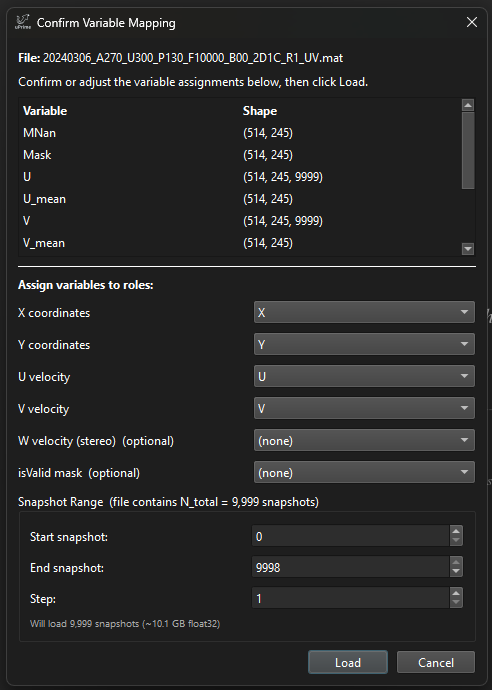
\includegraphics[width=0.65\linewidth]{fig_mat_dialog}
  \caption{\texttt{.mat} variable confirmation dialog. The top panel lists every variable in the file with its shape. Six dropdowns map the file variables to \href{https://cmdrryder.github.io/uPrime/}{uPrime}'s expected roles ($x$, $y$, $U$, $V$, $W$, isValid); auto-detected matches are pre-filled. The bottom panel sets the snapshot subset to load (start, end, step), with a live readout of the resulting count and estimated memory size. Click `Load` to confirm and start the actual data read.}
  \label{fig:matdialog}
\end{figure}

\paragraph{Snapshot subset.} The dialog includes Start, End, and Step spinboxes. They allow loading only a slice (e.g.\ snapshots 0--999) or a strided subsample (e.g.\ every 10th snapshot from 0 to 9999). The estimated in-memory size updates live. This is useful for preliminary inspection of very large files before committing to the full load.

\paragraph{Mask convention.} A `Mask convention` dropdown sits next to the isValid selector. The default, `1 = valid (uPrime default)`, matches the \texttt{.dat} convention. If your file uses the opposite convention (for example a \texttt{Mask} variable where 1 marks points to \emph{exclude}), select `1 = invalid (mask out)`. \href{https://cmdrryder.github.io/uPrime/}{uPrime} applies the chosen convention directly, with no auto-detection. After loading, the status bar warns if the resulting masked fraction is extreme (below 5\% or above 95\%); if that warning is unexpected, reload with the other convention.

\paragraph{Progress feedback.} For v7.3 files (HDF5), the read is chunked snapshot-by-snapshot and the progress bar advances determinately. For classic \texttt{.mat} files, the read is a single blocking call from \texttt{scipy.io}, so a busy indicator is shown along with the file size in the status bar. After the read, the status bar prints a confirmation listing the chosen variables and snapshot count, for example:

\begin{center}
\texttt{Loaded .mat: x=X, y=Y, u=U, v=V, w=(none), isValid=(none), N=1000 of 9999 (range 0:9990 step 10)}
\end{center}

```{tip}
For very large \texttt{.mat} files, save with \texttt{-v7.3} in MATLAB:\\
\texttt{save('dataset.mat', 'x', 'y', 'u', 'v', '-v7.3')}\\
This enables HDF5 chunked reading, which can show real per-snapshot progress and avoids loading the entire file in one blocking call.
```

```{warning}
A \texttt{.mat} file containing a single snapshot will be rejected before any data is read (Figure~\ref{fig:singlesnap}). Most \href{https://cmdrryder.github.io/uPrime/}{uPrime} modules require multiple snapshots to compute statistics; for a single snapshot only the field viewer is meaningful, which does not justify loading the file.
```

\begin{figure}[htbp]
  \centering
  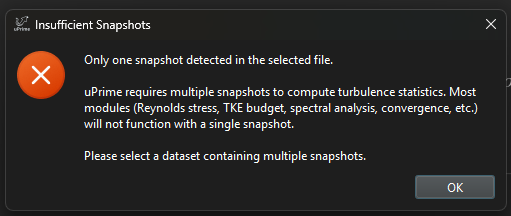
\includegraphics[width=0.55\linewidth]{fig_mat_singlesnap_error}
  \caption{Error dialog shown when a \texttt{.mat} file contains only one snapshot. The check is performed on the metadata before any data is loaded, so the error appears immediately regardless of the file size.}
  \label{fig:singlesnap}
\end{figure}

% ============================= CHAPTER 2 ==============================
